\begin{frame}{Issues in mobile environments}
	\begin{itemize}
		\item Even if a single packet is dropped due to a short disconnection,
		      standard TCP wrongly thinks that the loss was caused by
		      congestion and chokes the transmission.
		\item Thus, standard TCP's sender unnecessarily holds back,
		      (slow window growth), even
		      though the receiver often recoups quickly from a
                      short disconnection.
	\end{itemize}

	\begin{figure}
                \centering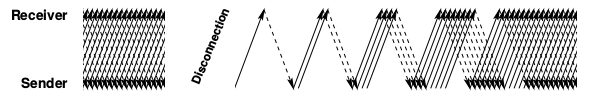
\includegraphics[scale=0.4]{freeze-disconn}
        \end{figure}

\end{frame}
